\chapter{Besselian Elements Method}
\label{chap:besselian}

\section{Introduction}

The Besselian method, classical for solar eclipses \citep{Meeus1998,Explanatory2013}, adapts elegantly to asteroid occultations.

\section{Fundamental Plane}

Define a plane perpendicular to star direction passing through Earth's center. Project asteroid shadow onto this plane.

\begin{figure}[htbp]
\centering
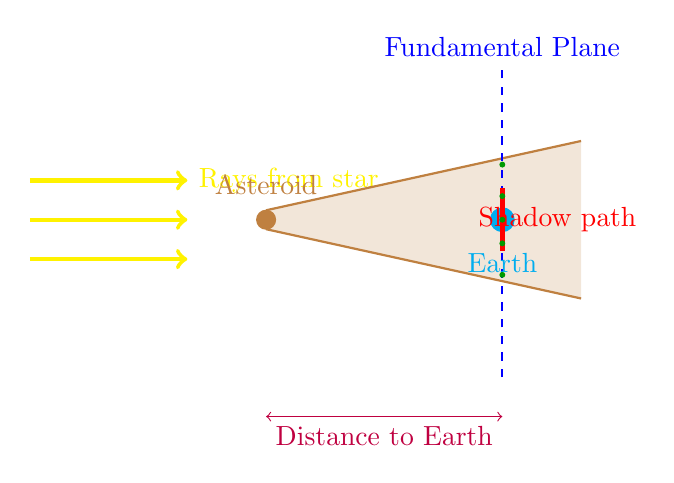
\begin{tikzpicture}[scale=1.0]
    % Star (far away)
    \draw[->,yellow,ultra thick] (-4,2) -- (-2,2) node[right] {Rays from star};
    \draw[->,yellow,ultra thick] (-4,1.5) -- (-2,1.5);
    \draw[->,yellow,ultra thick] (-4,1) -- (-2,1);
    
    % Asteroid
    \filldraw[brown] (-1,1.5) circle (0.12) node[above=0.2cm] {Asteroid};
    
    % Shadow cone
    \draw[brown,thick] (-1,1.62) -- (3,2.5);
    \draw[brown,thick] (-1,1.38) -- (3,0.5);
    \fill[brown,opacity=0.2] (-1,1.38) -- (3,0.5) -- (3,2.5) -- (-1,1.62) -- cycle;
    
    % Fundamental plane (perpendicular to star)
    \draw[blue,thick,dashed] (2,-0.5) -- (2,3.5);
    \node[blue] at (2,3.7) {Fundamental Plane};
    
    % Earth
    \filldraw[cyan] (2,1.5) circle (0.15) node[below=0.3cm] {Earth};
    
    % Shadow on plane
    \draw[red,ultra thick] (2,1.1) -- (2,1.9);
    \node[red] at (2.7,1.5) {Shadow path};
    
    % Observer positions
    \foreach \y in {0.8, 1.2, 1.5, 1.8, 2.2} {
        \filldraw[green!60!black] (2,\y) circle (0.03);
    }
    
    % Distance annotation
    \draw[<->,purple] (-1,-1) -- (2,-1) node[midway,below] {Distance to Earth};
\end{tikzpicture}
\caption{Besselian geometry. Asteroid shadow projected onto fundamental plane perpendicular to star direction. Observer positions on Earth map to points on this plane. Shadow path is straight line in this frame.}
\label{fig:besselian_geometry}
\end{figure}

\section{Besselian Elements}

Define coordinates $(\xi, \eta)$ in fundamental plane with origin at Earth's center:

\begin{align}
\xi &= \text{coordinate along shadow motion} \\
\eta &= \text{coordinate perpendicular to motion}
\end{align}

\textbf{Asteroid position in fundamental plane:}
\begin{align}
\xi_{\text{ast}}(t) &= \xi_0 + \dot{\xi} (t - t_0) \\
\eta_{\text{ast}}(t) &= \eta_0 + \dot{\eta} (t - t_0)
\end{align}

\textbf{Observer position:}
\begin{align}
\xi_{\text{obs}} &= \rho \cos\phi \sin(H + \lambda) \\
\eta_{\text{obs}} &= \rho (\sin\phi \cos\delta - \cos\phi \sin\delta \cos H)
\end{align}

where $\rho$ is geocentric distance, $H$ is hour angle, $(\phi, \lambda)$ is observer location.

\section{Occultation Condition}

Occultation occurs when:

\begin{equation}
\sqrt{(\xi_{\text{ast}} - \xi_{\text{obs}})^2 + (\eta_{\text{ast}} - \eta_{\text{obs}})^2} < R_{\text{shadow}}
\end{equation}

\textbf{Contact times:} Solve for $t$ when distance equals shadow radius.

\section{Advantages}

\begin{itemize}
    \item \textbf{Linear motion:} Shadow moves in straight line in $(\xi, \eta)$ plane
    \item \textbf{Simple geometry:} 2D problem instead of 3D
    \item \textbf{Fast:} Analytical closest approach calculation
    \item \textbf{Accurate:} No approximations in geometry
\end{itemize}

\section{Summary}

Besselian method reduces occultation geometry to 2D straight-line problem, enabling fast and precise predictions.

\textbf{References:}
\begin{itemize}
    \item Meeus (1998) \citep{Meeus1998}: solar eclipse calculations
    \item Explanatory Supplement (2013) \citep{Explanatory2013}: detailed formulation
\end{itemize}
